\documentclass[border=6pt]{standalone}
\usepackage{fontspec}
\setmainfont{lmroman10-regular.otf}[BoldFont=lmroman10-bold.otf, ItalicFont=lmroman10-italic.otf, BoldItalicFont=lmroman10-bolditalic.otf]
\setmonofont{lmmono10-regular.otf}[BoldFont=lmmonolt10-bold.otf, ItalicFont=lmmono10-italic.otf]
\usepackage{tikz}
\usetikzlibrary{arrows.meta,positioning,fit,calc,backgrounds}

% The README's figure. Build: xelatex open-lane-flow.tex, then pdftoppm -png -r 200 -singlefile open-lane-flow.pdf open-lane-flow
% The style and colours of Mech-Interp-Agent-level1's docs/figures/level1-flow.tex
\definecolor{agentfill}{RGB}{238,237,253}
\definecolor{agentdraw}{RGB}{90,82,181}
\definecolor{agenttext}{RGB}{43,39,104}
\definecolor{measfill}{RGB}{229,244,238}
\definecolor{measdraw}{RGB}{62,122,101}
\definecolor{meastext}{RGB}{24,64,50}
\definecolor{fixedfill}{RGB}{241,239,233}
\definecolor{fixeddraw}{RGB}{138,136,131}
\definecolor{fixedtext}{RGB}{51,51,51}
\definecolor{arrowc}{RGB}{112,112,112}

\tikzset{
  box/.style={rounded corners=2pt, line width=0.6pt, align=center, inner sep=5pt, font=\small},
  agent/.style={box, draw=agentdraw, fill=agentfill, text=agenttext},
  meas/.style={box, draw=measdraw, fill=measfill, text=meastext},
  fixed/.style={box, draw=fixeddraw, fill=fixedfill, text=fixedtext},
  opt/.style={dash pattern=on 3pt off 2pt},
  arr/.style={-{Stealth[length=2.2mm,width=1.6mm]}, draw=arrowc, line width=0.6pt},
  lab/.style={font=\small, text=fixedtext, align=left},
}
\newcommand{\tit}[1]{{\normalsize\bfseries #1}\\[1pt]}
\newcommand{\tool}[1]{{\normalsize\ttfamily\bfseries #1}\\[2pt]}

\begin{document}
\hyphenpenalty=10000 \exhyphenpenalty=10000
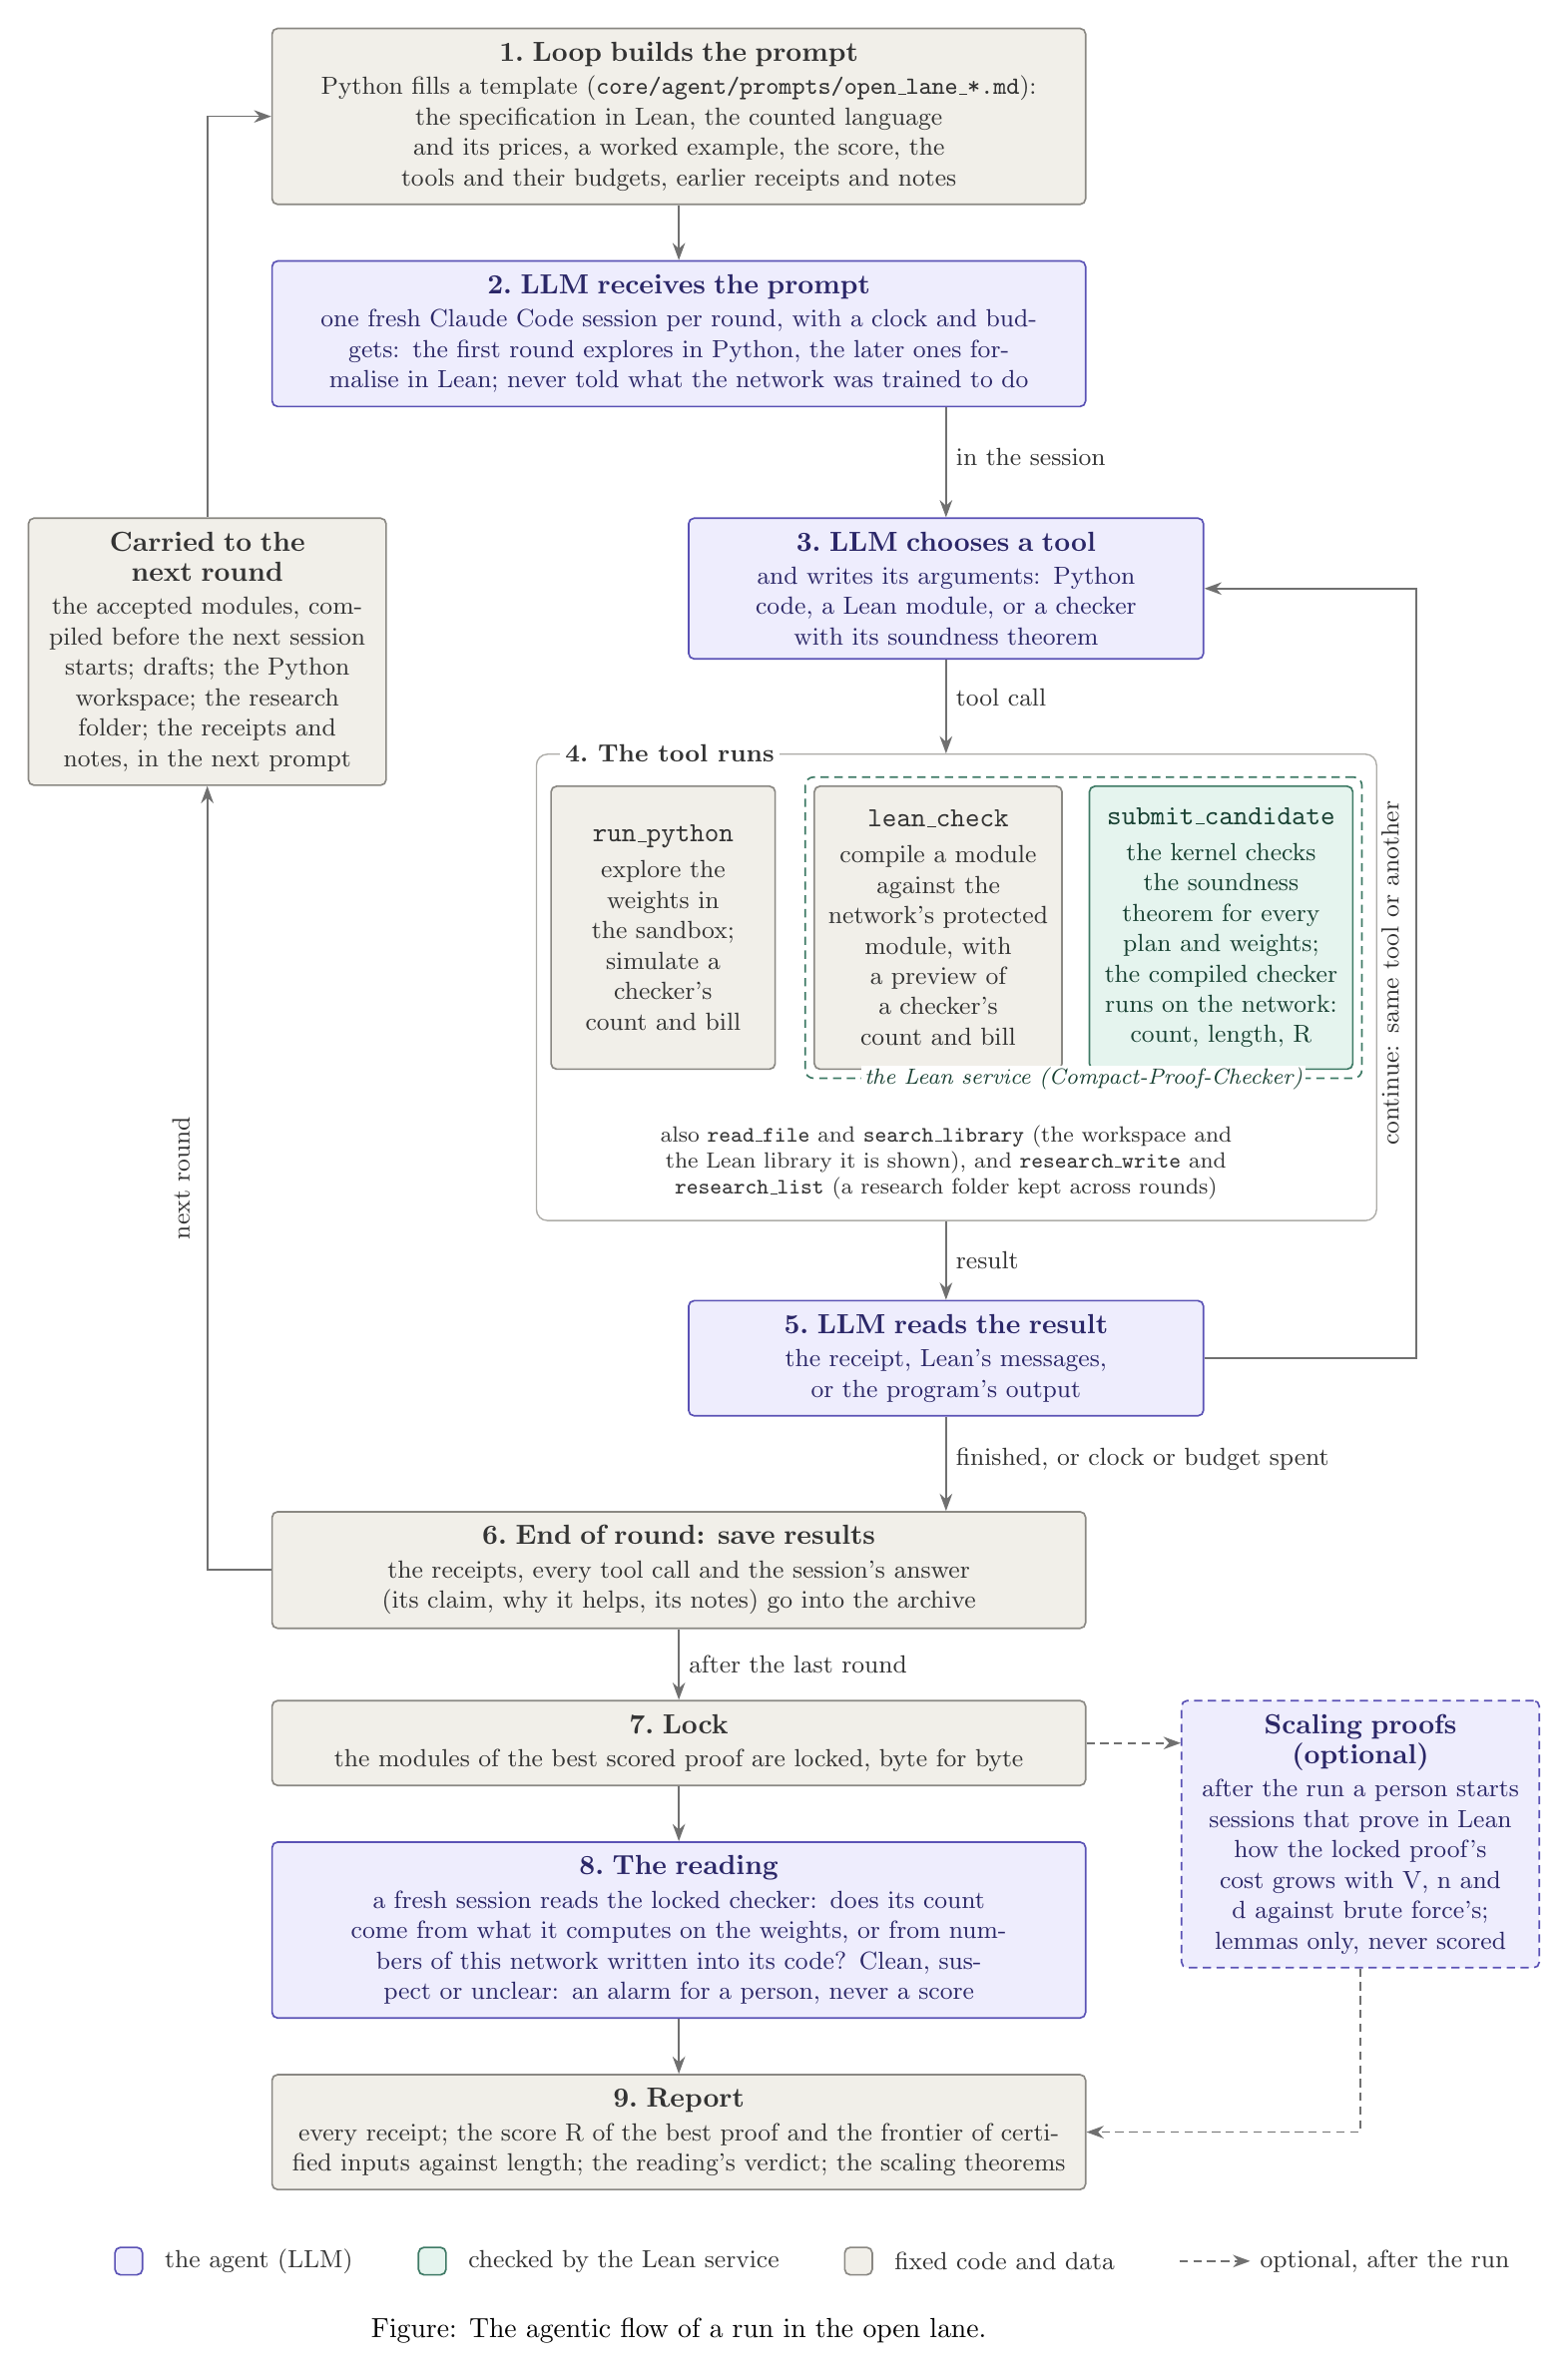
\begin{tikzpicture}

% 1, 2: the prompt, across the top
\node[fixed, text width=100mm] (p1) at (0,0) {\tit{1.\ Loop builds the prompt}
  Python fills a template (\texttt{core/agent/prompts/open\_lane\_*.md}): the specification in Lean, the counted
  language and its prices, a worked example, the score, the tools and their budgets,
  earlier receipts and notes};
\node[agent, text width=100mm, below=7mm of p1] (p2) {\tit{2.\ LLM receives the prompt}
  one fresh Claude Code session per round, with a clock and budgets: the first round explores in Python, the
  later ones formalise in Lean; never told what the network was trained to do};

% a session, on the right: steps 3 to 5
\coordinate (R) at (34mm,0);
\node[agent, text width=62mm, anchor=north] (p3) at ($(R |- p2.south)+(0,-14mm)$) {\tit{3.\ LLM chooses a tool}
  and writes its arguments: Python code, a Lean module, or a checker with its soundness theorem};
\node[fixed, text width=25mm, minimum height=36mm, anchor=north] (py) at ($(p3.south)+(-36mm,-16mm)$) {\tool{run\_python}
  explore the weights in the sandbox; simulate a checker's count and bill};
\node[fixed, text width=28mm, minimum height=36mm, anchor=north] (lc) at ($(p3.south)+(-1mm,-16mm)$) {\tool{lean\_check}
  compile a module against the network's protected module, with a preview of a checker's count and bill};
\node[meas, text width=30mm, minimum height=36mm, anchor=north] (sub) at ($(p3.south)+(35mm,-16mm)$) {\tool{submit\_candidate}
  the kernel checks the soundness theorem for every plan and weights; the compiled checker runs on the network:
  count, length, R};
\node[lab, text width=86mm, align=center, font=\footnotesize, anchor=north] (more) at ($(p3.south)+(0,-58mm)$)
  {also \texttt{read\_file} and \texttt{search\_library} (the workspace and the Lean library it is shown), and
  \texttt{research\_write} and \texttt{research\_list} (a research folder kept across rounds)};
\begin{scope}[on background layer]
  \node[draw=measdraw, opt, rounded corners=3pt, line width=0.6pt, fit=(lc)(sub), inner sep=3pt] (ver) {};
  \node[draw=fixeddraw!70, rounded corners=4pt, line width=0.5pt, fit=(py)(sub)(ver)(more), inner xsep=5pt,
        inner ysep=6pt, yshift=2pt] (tools) {};
\end{scope}
\node[fill=white, inner sep=2pt, font=\small\bfseries, text=fixedtext, anchor=west] at ($(tools.north west)+(3mm,0)$) {4.\ The tool runs};
\node[font=\footnotesize\itshape, text=meastext, fill=white, inner sep=1pt] at (ver.south) {the Lean service (Compact-Proof-Checker)};
\node[agent, text width=62mm, anchor=north] (p5) at ($(R |- tools.south)+(0,-10mm)$) {\tit{5.\ LLM reads the result}
  the receipt, Lean's messages, or the program's output};

% 6 to 9: below, across
\node[fixed, text width=100mm, anchor=north] (p6) at ($(0,0 |- p5.south)+(0,-12mm)$) {\tit{6.\ End of round: save results}
  the receipts, every tool call and the session's answer (its claim, why it helps, its notes) go into the archive};
\node[fixed, text width=100mm, below=9mm of p6] (p7) {\tit{7.\ Lock}
  the modules of the best scored proof are locked, byte for byte};
\node[agent, text width=100mm, below=7mm of p7] (p8) {\tit{8.\ The reading}
  a fresh session reads the locked checker: does its count come from what it computes on the weights, or from
  numbers of this network written into its code? Clean, suspect or unclear: an alarm for a person, never a score};
\node[fixed, text width=100mm, below=7mm of p8] (p9) {\tit{9.\ Report}
  every receipt; the score R of the best proof and the frontier of certified inputs against length; the
  reading's verdict; the scaling theorems};

% on the left: what the next round starts from, and the scaling proofs after the run
\coordinate (L) at (-60mm,0);
\node[fixed, text width=42mm, anchor=north] (keep) at ($(L |- p3.north)+(0,0)$) {\tit{Carried to the next round}
  the accepted modules, compiled before the next session starts; drafts; the Python workspace; the research
  folder; the receipts and notes, in the next prompt};
\node[agent, opt, text width=42mm, anchor=north west] (sc) at ($(p7.north east)+(12mm,0)$) {\tit{Scaling proofs (optional)}
  after the run a person starts sessions that prove in Lean how the locked proof's cost grows with V, n and d
  against brute force's; lemmas only, never scored};

% arrows
\draw[arr] (p1) -- (p2);
\draw[arr] ($(p2.south)+(34mm,0)$) -- node[lab, right, pos=0.45] {in the session} (p3.north);
\draw[arr] (p3.south) -- node[lab, right, pos=0.4] {tool call} (p3.south |- tools.north);
\draw[arr] (p3.south |- tools.south) -- node[lab, right, pos=0.5] {result} (p5.north);
\coordinate (loop) at ($(tools.east)+(5mm,0)$);
\draw[arr] (p5.east) -| (loop |- p5.east) |- node[lab, pos=0.25, rotate=90, anchor=south, yshift=1mm] {continue: same tool or another} (p3.east);
\draw[arr] (p5.south) -- node[lab, right, pos=0.45] {finished, or clock or budget spent} (p5.south |- p6.north);
\draw[arr] (p6.west) -| node[lab, pos=0.75, rotate=90, anchor=south, yshift=1mm] {next round} (keep.south);
\draw[arr] (keep.north) |- (p1.west);
\draw[arr] (p6) -- node[lab, right, pos=0.5] {after the last round} (p7);
\draw[arr] (p7) -- (p8);
\draw[arr] (p8) -- (p9);
\draw[arr, opt] (p7.east) -- (p7.east -| sc.west);
\draw[arr, opt] (sc.south) |- (p9.east);

% legend and caption
\node[agent, minimum width=3.5mm, minimum height=3.5mm, inner sep=0pt] (l1) at ($(p9.south)+(-70mm,-9mm)$) {};
\node[lab, right=1.5mm of l1] (t1) {the agent (LLM)};
\node[meas, minimum width=3.5mm, minimum height=3.5mm, inner sep=0pt, right=7mm of t1] (l2) {};
\node[lab, right=1.5mm of l2] (t2) {checked by the Lean service};
\node[fixed, minimum width=3.5mm, minimum height=3.5mm, inner sep=0pt, right=7mm of t2] (l3) {};
\node[lab, right=1.5mm of l3] (t3) {fixed code and data};
\draw[arr, opt] ($(t3.east)+(7mm,0)$) -- ++(9mm,0) node[lab, right] {optional, after the run};
\node[font=\normalsize, anchor=north] at ($(p9.south)+(0,-15mm)$) {Figure: The agentic flow of a run in the open lane.};
\end{tikzpicture}
\end{document}
